% ======================================================================
\chapter[DEVELOPMENT AND IMPLEMENTATION]{Development and Implementation}
\label{ch:impl}
% ======================================================================

\section{Introduction to the Tools}

The project is a software project, and nearly all of it was written in Python.

\paragraph{PyTorch.} All networks were built and trained with PyTorch \cite{paszke2019pytorch}. We used its automatic mixed precision: bfloat16 on the laptop's RTX~4050, which supports it natively, and float16 with dynamic loss scaling \cite{micikevicius2018amp} on Kaggle's T4 GPUs, which do not. For the two-GPU runs on Kaggle we used PyTorch's distributed data parallel mode, which keeps one copy of the model on each GPU and averages the gradients after every update.

\paragraph{timm.} The PyTorch Image Models library \cite{wightman2019timm} provided the pretrained encoders (ConvNeXt-Tiny, EfficientNet-B0, EfficientNetV2-S and ResNet-18d) with a common interface, so a backbone could be swapped by changing one name. Its implementation of the weight EMA was also used.

\paragraph{pydicom and image decoders.} DICOM files were read with pydicom \cite{mason_pydicom}. The local copy of the data was uncompressed, but the competition stated that test files might use JPEG-Lossless or JPEG~2000 compression \cite{dicom_standard}. pydicom needs separate decoder packages for these formats (pylibjpeg with its libjpeg and OpenJPEG plug-ins), and it looks for them only when it is first imported. This detail caused one of the more serious pipeline defects found in the project (Section~\ref{sec:impl-mil}).

\paragraph{Hugging Face Transformers and bitsandbytes.} The local report labeller ran the Qwen3-4B-Instruct model \cite{yang2025qwen3} through the Transformers library \cite{wolf2020transformers}. The model weights were quantised to 4-bit NormalFloat (NF4) with bitsandbytes \cite{dettmers2023qlora,bitsandbytes} so that the model fits on the 6~GB laptop GPU next to its key--value cache. The first labeller of the project used the vLLM serving engine \cite{kwon2023vllm} on Kaggle instead.

\paragraph{scikit-learn, NumPy and pandas.} These were used for data tables, fold assignment and metric computation. For bootstrap confidence intervals, which need thousands of AUC evaluations, we computed the AUC with the rank-sum (Mann--Whitney) formula, which is equivalent to Equation~\eqref{eq:auc}, and checked it against scikit-learn's implementation.

\paragraph{Hardware.} The laptop described in Table~\ref{tab:equipment} did all label generation, all training of our own 2.5D model and all local evaluation. Kaggle's free notebooks with two T4 GPUs were used for the submissions and for the larger post-competition models.

\section{Other Supporting Tools}

\begin{itemize}[leftmargin=1.4em]
\item \textbf{Git} kept the history of the code. After the data audit, data-derived files (labels, caches, predictions) were excluded from version control because of the data licence.
\item \textbf{The Kaggle command-line client} \cite{kaggle_cli} was used to download public datasets, push notebooks, submit and read the submission history. We wrapped it in a small script that reads the API token from its file into the child process only, never prints it, and refuses any write operation that had not been explicitly approved.
\item \textbf{Notebook generators.} Kaggle notebooks were generated from the tested Python modules by build scripts, and a local test executed each generated notebook from start to end in a fresh interpreter before it was uploaded.
\item \textbf{A run queue} on the laptop started training runs one after another, resumed a run from its last checkpoint after an interruption, and kept a second GPU job from starting while one was running.
\item \textbf{Hand-over scripts} on the laptop watched Kaggle runs and, when a run ended, downloaded its weights, built the next notebook and submitted it. They keep their progress in a state file so that a restart can never submit twice.
\item \textbf{FastAPI, React, Vite and three.js} were used for the workstation (Section~\ref{sec:impl-demo}).
\item \textbf{matplotlib} produced every chart in this report from aggregate result tables, and the report itself was typeset in \LaTeX.
\end{itemize}

\section{Implementation}
\label{sec:implementation}

This section follows the project through its six stages in the order in which they happened.

% ----------------------------------------------------------------------
\subsection{Stage 1: First labels and frozen-feature baselines}
\label{sec:impl-stage1}

\subsubsection{Literature survey and first plan} We began by reading the knee MRI literature summarised in Section~1.1.4 and by running two public implementations of MRNet on its own dataset to understand the per-slice encoder and pooling design. Our first architecture plan used a frozen DINOv2-small encoder \cite{oquab2024dinov2} on every slice and a small transformer with ``region-guided'' attention heads, one head for each anatomical group of findings (ligaments, menisci, compartments, fluid, bone). Before any of this could be trained, however, the 4,349 report-only studies needed labels.

\subsubsection{First LLM labeller} The reports are written in nine languages, so a multilingual model was needed. Our first attempt served Qwen2.5-14B-Instruct \cite{qwen2025qwen25} with vLLM on Kaggle's two T4 GPUs and ran out of memory. In half precision the 14-billion-parameter model alone needs about 28~GB, before any key--value cache is allocated. An English medical model, Llama3-OpenBioLLM-8B, was considered and rejected because of its weak handling of Spanish and Dutch reports. The working version used Qwen2.5-7B-Instruct with vLLM, with the memory utilisation limited to 85\%, a maximum context of 4,096 tokens and eager execution. The prompt contained a small Spanish and Dutch glossary, the report text was cut to 1,200 characters, and the model was asked to write a JSON object with twelve probabilities. A 4-bit (AWQ) version of the 14B model was run the same way later.

These labels were combined with two report-derived label sets that other participants had published on Kaggle (called P1 and P2 in this report), and with a third public file, by a consensus procedure inspired by Dawid--Skene \cite{dawid1979} and confident learning \cite{northcutt2021cl}. The weight of each source was set from its agreement with the 58 gold studies.

\subsubsection{Frozen-feature image models} The first image models kept the encoder frozen. Version~1 took twelve slices from one series per plane, encoded each slice with an ImageNet-pretrained EfficientNet-B0 \cite{tan2019effnet}, pooled the slices of each plane with attention and passed the three plane vectors to a small network. Caching the frozen features cut the training time from 441~s to about 5~s per epoch. Version~1 read its images from a preprocessed archive published by another participant. Its first submission scored 0.500 on the public leaderboard, the score of a random guess, because the archive did not contain the hidden test studies and the notebook therefore had no real images to work from. Version~2 replaced the archive with our own DICOM pipeline (slice ordering by Equation~\eqref{eq:sliceorder} and percentile normalisation by Equation~\eqref{eq:norm}) and scored \textbf{0.775 public / 0.755 private}. Two further versions, one with mirroring of right knees, up to three series per plane and region-guided heads, and one with a frozen DINOv2 encoder, did not do better on our validation.

All four versions chose their best epoch by the AUC on the gold studies of the validation fold, and gold studies were in the training folds with eight times the normal weight. Their reported gold scores were therefore optimistic. We did not see this at the time; it was found in the audit of Stage~2.

% ----------------------------------------------------------------------
\subsection{Stage 2: Data and label audit, and a new local labeller}
\label{sec:impl-audit}

The jump from 0.500 to 0.775 was the result of a bug fix, and we had no reliable way to tell whether later changes helped. We therefore stopped and audited the whole data and label pipeline before building anything new.

\subsubsection{Defects found} The audit read all 819,078 DICOM headers, all reports and every label file. Table~\ref{tab:defects} lists the problems that mattered. Several of them were silent, in the sense that the pipeline ran without errors and produced plausible numbers.

\begin{table}[htbp]
\centering\footnotesize\setstretch{1}
\caption{Defects found in the audit of the first pipeline}
\label{tab:defects}
\begin{tabularx}{\textwidth}{L{3.9cm} Y L{2.6cm}}
\toprule
Defect & Evidence & Consequence \\
\midrule
Constant voter in the consensus & one ``public pseudo-label'' file held exactly 0.5 for all 52,188 unlabelled cells; with a $\geq0.5$ rule it voted ``positive'' everywhere & corrupted consensus \\
Silent 0.5 fallback & a failed JSON parse would write 0.5 for all twelve findings without a flag; in the final 7B file 1,744 cells were exactly 0.5, which a $\geq0.5$ rule counts as positive & uncertain cells counted as positives \\
Report truncation & the 1,200-character cut shortened 37.7\% of all reports and half of the gold reports, often removing the conclusion & missed findings \\
Character corruption & 95\% of Greek reports used the micro sign in place of the Greek letter mu & unreadable Greek text \\
Gold used for selection & consensus weights and best epochs chosen on gold; gold rows also trained on & optimistic gold scores \\
Incomplete laterality & only studies tagged exactly ``R'' were mirrored (about half of the right knees) & medial/lateral mixed up \\
Silent zero-fill & a plane whose slices failed to decode became a blank image & corrupted test inputs \\
Missing decoder & no JPEG-Lossless decoder installed, while the hidden test may be compressed & blank test planes \\
Protocol shortcut & studies with a series named ``ACL'' were ACL-positive in 50.6\% vs 17.3\% of reports & shortcut risk \\
\bottomrule
\end{tabularx}
\end{table}

The audit also measured how the report-derived labels differ from the gold labels. Figure~\ref{fig:labels}(a) compares the share of studies called positive by each label source. Report-derived labels mark synovitis in about 12\% of studies, while the gold readers mark it in 47\% of theirs; fractures and lateral meniscal tears show the same pattern. Part of this gap is the enrichment of the gold set, but the per-finding pattern is not uniform. The gold readers saw synovitis and fractures that the reports never mention. The figure also includes the two image-read label sets that became available after the competition (Section~\ref{sec:impl-post}); they show the opposite problem for findings with a size or grade threshold, such as MCL injury, lateral OA, PF OA and effusion, which our report labels call far more often than an image reader does.

\begin{figure}[htbp]
\centering\setstretch{1}
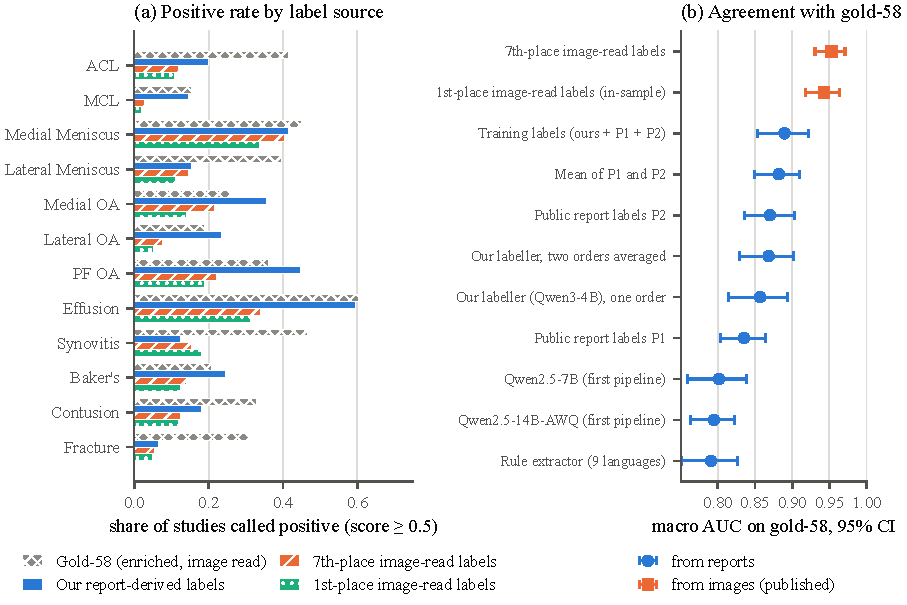
\includegraphics[width=\textwidth]{fig_labels.pdf}
\caption[Label prevalence and agreement with gold-58]{Label quality: (a) share of studies called positive by each label source (gold-58 is enriched, so its rates are not population rates), and (b) macro AUC of each label source against the gold-58 labels with 95\% bootstrap confidence intervals}
\label{fig:labels}
\end{figure}

\subsubsection{The forced-choice labeller} The new labeller follows the design of Section~\ref{sec:design-labels}. It runs Qwen3-4B-Instruct-2507 in 4-bit NF4 on the laptop GPU and reads the full report after Unicode normalisation and the Greek character repair. The prompt was developed on 60 non-gold studies and frozen before its first evaluation on gold. Two engineering problems had to be solved to make it fast enough. First, the Transformers library computes output logits over the whole vocabulary for every prompt position by default, which for an 8,000-token prompt needed 3.6~GB and pushed the card into shared system memory; asking for the logits of the last position only removed the problem. Second, the long system prompt is identical for every report, so its key--value cache was computed once and reused, which made the labeller about twelve times faster. On 96 test items the cached and uncached versions gave the same answers except for near-ties. The final labeller processed 0.94--1.6 studies per second with a peak of 4.4~GB of GPU memory, and each full pass over the 4,407 reports took about 75 minutes. All 4,407 reports were processed without a single failure, and the probability mass on the five answer letters was at least 0.995 everywhere. A rule-based extractor with negation handling for all nine languages was written as well, mainly to give an independent second opinion and evidence spans.

\subsubsection{Label quality against gold} Figure~\ref{fig:labels}(b) shows the macro AUC of every label source against the 58 gold studies. The forced-choice labeller scored 0.857, against 0.802 for the first Qwen2.5-7B pipeline; the paired difference was $+0.055$ with a 95\% confidence interval of $[+0.012, +0.093]$. Averaging its two item orders raised it to \textbf{0.868}, which is the score of our own labeller. The training labels of Equation~\eqref{eq:teacher}, the mean of our labeller and the public sets P1 and P2, reached 0.890 $[0.853, 0.922]$, the best of all report-based sources. As noted in Section~\ref{sec:design-labels}, part of P1 matches the gold labels exactly, so this figure may be slightly optimistic. The rule extractor was the weakest source at 0.791 and was not used for training. Every labeller had its lowest AUC on synovitis (0.67--0.74), and the strongest labellers called about two thirds of the gold-negative effusions positive. Both patterns come from differences between the reports and the images, which no report reader can fix.

\subsubsection{Effect of the labels on the image model} To answer this, the frozen-feature model of version~2 was retrained from scratch on each label set, with fixed epochs, five seeds, and gold used only for the final score. Table~\ref{tab:downstream} shows the result. Training on report-derived labels gave 0.75--0.78 on gold, while training on the 58 gold studies alone gave only 0.51--0.59. The labels were clearly useful. But the differences between label sets were small, within about 0.03, and masking the ``not mentioned'' cells made results worse. With frozen features the image model limited the result more than the labels did, so Stage~3 focused on the image model.

\begin{table}[htbp]
\centering\footnotesize\setstretch{1}
\caption[Downstream test of label sets with frozen features]{Downstream test: the frozen-feature model retrained on different label sets, scored on gold-58 (mean of five seeds)}
\label{tab:downstream}
\begin{tabular}{L{8.8cm}C{4.2cm}}
\toprule
Training labels & Gold-58 macro AUC [95\% CI] \\
\midrule
Final teacher (order-averaged LLM + two public sets) & 0.782 [0.735, 0.827] \\
Consensus of the first pipeline & 0.772 [0.725, 0.818] \\
Qwen2.5-7B labels of the first pipeline & 0.761 [0.709, 0.812] \\
Final teacher with ``not mentioned'' cells masked & 0.758 [0.707, 0.804] \\
Rule extractor & 0.747 [0.695, 0.798] \\
The 58 gold studies only (leave-one-out) & 0.51--0.59 \\
\bottomrule
\end{tabular}
\end{table}

% ----------------------------------------------------------------------
\subsection{Stage 3: The fine-tuned 2.5D multiple-instance model}
\label{sec:impl-mil}

\subsubsection{Pipeline corrections} The design of Section~\ref{sec:design-mil} was implemented as a set of Python modules for study indexing, decoding, data loading, the model, training and prediction. Before training, the defects of Table~\ref{tab:defects} that concern images were fixed and tested:
\begin{itemize}[leftmargin=1.4em]
\item \emph{Laterality.} The side is now taken from the tag or, failing that, from the coronal and axial geometry; disagreements between tag and geometry fell from 57 to 28 studies. After normalisation, the correlation between the mean left-knee image and the mean right-knee image rose from 0.869 to 0.988 in the coronal plane and from 0.950 to 0.988 in the sagittal plane.
\item \emph{Decoding.} A series that fails to decode falls back to the next candidate or is masked; it is never filled with zeros. A single unreadable slice at either end of a long series is dropped and recorded. If more than 2\% of the studies fail, the run stops.
\item \emph{Kaggle environment.} Kaggle's image used Python 3.13, for which no decoder wheels had been prepared, and pydicom finds its decoder plug-ins only at its first import. Without a fix, every compressed test study would have been decoded to nothing. We shipped decoder wheels for Python 3.10--3.14 in a private dataset and installed them before the first import of pydicom; the notebook checks for all four decoders before it starts.
\item \emph{Parity.} The preprocessing used for training and for inference was shown to give bit-identical arrays on 51 local series.
\end{itemize}

\subsubsection{Training} All training of this model ran on the laptop. The recipe is summarised in Table~\ref{tab:milrecipe}. One run of eight epochs on the four training folds (3,479 studies) took about 57 minutes at a steady 8.4 studies per second, with a peak of 3.8~GB of GPU memory. Long runs heated the GPU to its thermal limit and reduced its clock from about 3.1 to 2.0~GHz, and all timings in this report are at that throttled speed. Each run saved a complete checkpoint every epoch and could be resumed after the laptop slept or restarted.

\begin{table}[htbp]
\centering\footnotesize\setstretch{1}
\caption{Training recipe of the 2.5D multiple-instance model}
\label{tab:milrecipe}
\begin{tabularx}{\textwidth}{L{4.0cm} Y}
\toprule
Item & Setting \\
\midrule
Input & 3 series (sagittal, coronal, axial; fluid-sensitive first) $\times$ 8 windows $\times$ 3 slices, 224 $\times$ 224 pixels \\
Encoder & ConvNeXt-Tiny, ImageNet-22k pretrained and ImageNet-1k fine-tuned; drop-path 0.1 \\
Head & projection to 384 dimensions, slot and position embeddings, 12 attention heads, 12 linear outputs (28.4~M parameters in total) \\
Labels and loss & soft teacher labels (Equation~\ref{eq:teacher}), binary cross-entropy (Equation~\ref{eq:bce}); gold studies excluded \\
Optimiser & AdamW, learning rate $1\times10^{-4}$ for the encoder and $5\times10^{-4}$ for the head, weight decay 0.05 \\
Schedule & 0.5 epoch linear warm-up, cosine decay to zero at epoch 8; gradient-norm clipping at 1.0 \\
Batch & 2 studies with 2 accumulation steps (effective batch of 4 studies) \\
Precision and EMA & bfloat16 autocast on the laptop, float16 on T4; EMA decay 0.999 \\
Augmentation & one affine transform per series (rotation $\pm10^\circ$, scale $\pm10\%$, shift $\pm6\%$), gamma $\pm20\%$, gain $\pm10\%$, random window centres; no left--right flips, which would undo the laterality normalisation \\
\bottomrule
\end{tabularx}
\end{table}

\subsubsection{Results on the held-out fold} Figure~\ref{fig:curves}(a) shows the validation curves. Fine-tuning the encoder (run E1) reached a macro AUC of \textbf{0.882} $[0.873, 0.891]$ on the 870 studies of our fold~0, against 0.792 for the frozen-feature design re-run under the same protocol (E0, best of its three seeds; Figure~\ref{fig:curves}a shows their mean). The paired gain was $+0.090$ $[+0.079, +0.101]$, and every one of the twelve findings improved. It was the largest gain from any change to our own model. E0 was trained on our four training folds only and without averaging over seeds, which is why its gold score below (0.753) is lower than the 0.782 of the same frozen design in Table~\ref{tab:downstream}.

\begin{figure}[htbp]
\centering\setstretch{1}
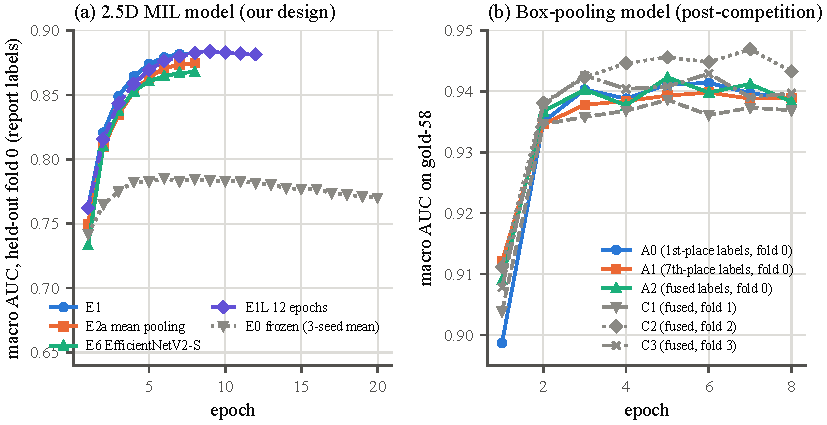
\includegraphics[width=\textwidth]{fig_curves.pdf}
\caption[Validation curves of the 2.5D and box-pooling models]{Validation curves: (a) our 2.5D model and its variants on our fold 0, scored against report-derived labels (E0 is the mean of three seeds); (b) the post-competition box-pooling runs on gold-58}
\label{fig:curves}
\end{figure}

\subsubsection{Ablations} We then tested one change at a time against E1, with the decision rule written down before the results were seen. Figure~\ref{fig:ablation} shows the paired differences on the held-out fold and on gold-58. A second run of the unchanged recipe with another seed differed from E1 by $+0.003$ on the held-out fold and by $+0.013$ on gold, which sets the scale of noise. Against that scale, none of the seven design changes was a clear improvement. A transformer layer over the tokens added $+0.002$ at 1.17 times the cost, and six series instead of three, a finer 0.6~mm pixel grid and twelve epochs made no clear difference. Mean pooling ($-0.008$), confidence-weighted labels ($-0.005$) and an EfficientNetV2-S encoder \cite{tan2021effnetv2} ($-0.015$) were worse, and on gold-58 all three pointed the same way. The eighth row of the figure, E1p, is a bug fix described below. The design of Section~\ref{sec:design-mil} was therefore kept as it was.

\begin{figure}[htbp]
\centering\setstretch{1}
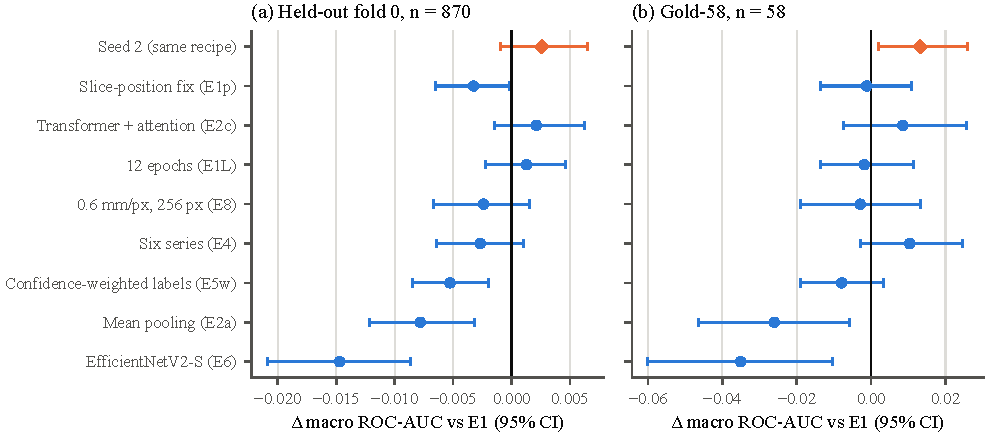
\includegraphics[width=\textwidth]{fig_ablation.pdf}
\caption[Single-change ablations of the 2.5D model]{Single-change ablations of the 2.5D model, as paired differences in macro AUC from run E1: (a) on the 870 studies of our fold 0 and (b) on gold-58; the orange point is a second seed of the unchanged recipe and shows the noise level}
\label{fig:ablation}
\end{figure}

\subsubsection{Where the model looks} Because each finding has its own attention distribution, the attention weights show where the model gathers its evidence, even though it was never told where any finding is. We averaged them over 300 validation studies (Figure~\ref{fig:attention}). The MCL head puts half of its weight on the coronal plane, where the collateral ligaments are seen along their length. The Baker's cyst head prefers coronal and axial slices, and the effusion head the axial plane. In the sagittal plane, the lateral meniscus head looks at the lateral end of the stack (mean position 0.39) and the medial meniscus head at the medial end (0.64). This separation can only appear if the laterality normalisation works. The same analysis exposed one more defect. The slice-position input was mirrored for right-knee sagittal series. It was fixed (run E1p) and the fix was kept as a correctness change; its effect on the score ($-0.003$) was no larger than the difference between two seeds.

\begin{figure}[htbp]
\centering\setstretch{1}
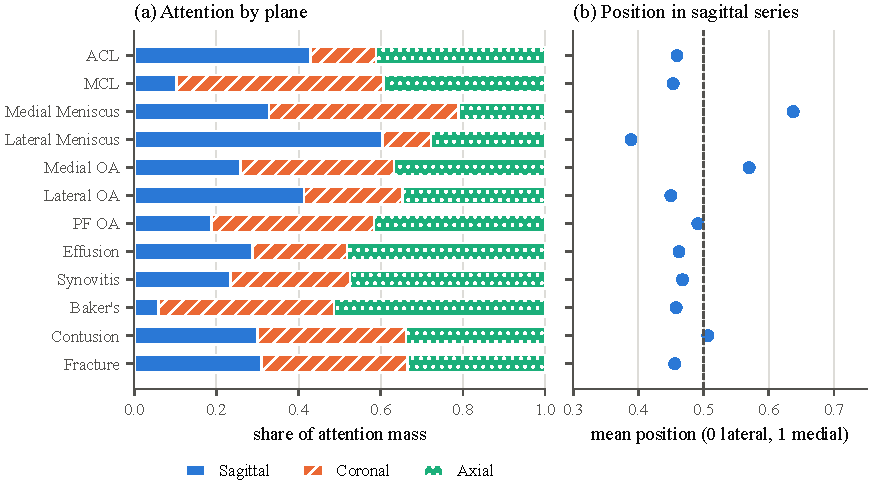
\includegraphics[width=\textwidth]{fig_attention.pdf}
\caption[Attention of the 2.5D model by plane and position]{Where the per-finding attention of the 2.5D model goes, averaged over 300 validation studies: (a) share of the attention on each plane and (b) mean position of the attention within the sagittal series}
\label{fig:attention}
\end{figure}

\subsubsection{Test-time averaging and the final ensemble} Larger sets of windows at test time did not help, but averaging two sets of eight windows, the second shifted by half a step, gave a small consistent gain of $+0.0017$ $[+0.0001, +0.0033]$ and was adopted. The final package contained three models with the locked recipe, F1, F2 and F3, trained with seeds 42, 7 and 11 on all 4,349 report-labelled studies (84--86 minutes each). Only after this choice was fixed was gold-58 scored, once, for all runs together. The final ensemble reached \textbf{0.906} $[0.877, 0.932]$ on gold-58, against 0.753 for the frozen-feature design (Figure~\ref{fig:gold}). Synovitis was the clear outlier at 0.680, close to the 0.68--0.74 of the report labels themselves. The model had learned what the reports say about synovitis rather than what the images show.

\begin{figure}[htbp]
\centering\setstretch{1}
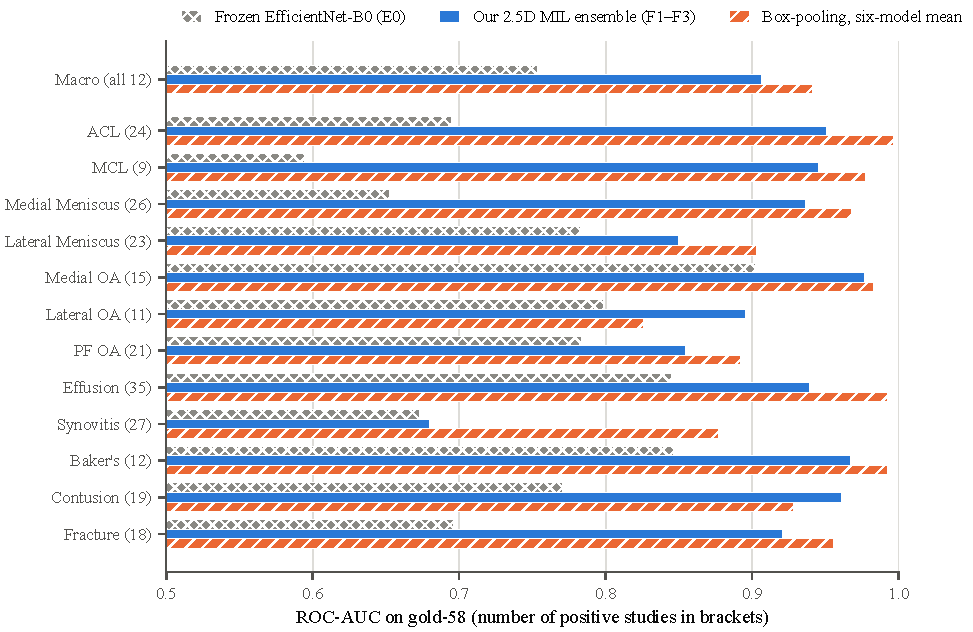
\includegraphics[width=\textwidth]{fig_gold_per_finding.pdf}
\caption[Per-finding AUC on gold-58]{Per-finding AUC on gold-58 for the frozen-feature baseline, our final 2.5D ensemble (Stage 3) and the six-model box-pooling ensemble (Stage 5)}
\label{fig:gold}
\end{figure}

\subsubsection{Submission} Measured end to end on the laptop, the three-model package with test-time averaging needed 1.9~s per study, about 42 minutes for 1,300 studies, of which 70--80\% was DICOM reading and decoding. The submission scored \textbf{0.927 on the public leaderboard and 0.916 on the private leaderboard}. A later variant added a fourth model, E9, trained at higher resolution (0.365~mm per pixel with a 320-pixel crop). It had gained $+0.005$ $[+0.001, +0.009]$ on the held-out fold, which is within the 0.003--0.006 differences we had seen between repeated runs of the same recipe, and on the leaderboard it scored 0.928 public and 0.915 private, the same as before. A round of self-training on the model's own out-of-fold predictions was also trained but never scored on the leaderboard, so we make no claim about it.

% ----------------------------------------------------------------------
\subsection{Stage 4: The competition endgame}
\label{sec:impl-endgame}

\subsubsection{The gap} With five days left, the best public notebooks scored 0.954--0.958 on the public leaderboard against our 0.927. Every public notebook above 0.950 used a CoAtNet \cite{dai2021coatnet} model that its author had trained with 2,399 additional knees from the OAI \cite{nevitt_oai,nartaa_swa}. Our own experiments in Stage~3 had found no change to our model that moved the held-out score beyond noise, and closing a gap of 0.03 with a single model of our own in five days was not realistic. We therefore changed strategy for the final submissions. Instead of one model of our own, we built ensembles around the strongest public models (Table~\ref{tab:public}) and spent our effort on checking, combining and re-engineering them.

\begin{table}[htbp]
\centering\footnotesize\setstretch{1}
\caption[Public models used in the competition endgame]{Public models and notebooks used in the competition endgame, with the extra data in their training as traced by us and their macro AUC when we ran them on gold-58}
\label{tab:public}
\begin{tabularx}{\textwidth}{L{2.0cm} L{2.6cm} Y C{1.3cm} L{2.6cm}}
\toprule
Model & Published by & Network and extra training data & Gold-58 & Used in \\
\midrule
CoAtNet & nartaa \cite{nartaa_swa} & CoAtNet at 384 pixels; 2,399 extra knees from the OAI & 0.923 & every pick \\
S6 & heliosli \cite{heliosli_compact} & ConvNeXt with an anatomy crop model trained on SKM-TEA & 0.927 & A-strict, final-strict \\
s6fall & nartaa \cite{nartaa_s6fall} & S6 retrained on all report-labelled studies & 0.931 & final-strict, final-max \\
R6 & heliosli, re-hosted by rostigor \cite{rostigor_r6} & ConvNeXt at 384 pixels with the same SKM-TEA crop model; auxiliary task on fastMRI+ (inferred from its trainer) & 0.937 & final-max \\
\midrule
\multicolumn{5}{L{15.6cm}}{Notebooks used as the base of our picks: heliosli's CoAtNet + S6 blend \cite{heliosli_blendgold} (A-strict) and goodpjw2008's CoAtNet + R6 pipeline \cite{goodpjw_coatnet_nb} (final-max).} \\
\bottomrule
\end{tabularx}
\end{table}


\subsubsection{Provenance checks} External data was allowed only if it was freely and equally available. We traced the training data of every public model we considered. The CoAtNet models used the OAI, which needs only a registration and a click-through data-use agreement; in our reading this met the organisers' general test, although they gave no ruling on individual datasets. A model called R6 and its successor R7 turned out to use an auxiliary task trained on fastMRI+ \cite{zhao2022fastmriplus}, whose access requires an institutional affiliation. The crop model of another family used SKM-TEA \cite{desai2021skmtea}. One of the two final picks was kept free of fastMRI-derived models, so that the team had one entry that did not depend on that question.

\subsubsection{Running every model ourselves} Before any model went into a submission, we ran it on the laptop with its author's code and scored it on gold-58 (Table~\ref{tab:public}). This needed some porting. One fast DICOM reader used a system call that exists only on Unix; on Windows the error was swallowed and every volume came back empty without any message. We patched the reader, checked that its output was byte-identical to the original on a reference set, and added a check that every volume contains slices. The local runs also gave us the cost of each model, which decided what could fit in the nine-hour limit: about 3~s per study for the CoAtNet, 6.5~s for s6fall, 19~s for S6 and 54--62~s for R6, which runs four folds with mirrored copies.

\subsubsection{Designing the blends} The ensembles themselves were ours. For each submission we fixed the members and their weights in writing before it was scored. The fastMRI-free pick, final-strict, combines the CoAtNet, S6 and s6fall with weights 0.5, 0.25 and 0.25; before it ran we predicted 0.955--0.956 on the public leaderboard, and it scored 0.956. For A-strict+ we replaced the R6 stage of the strongest public notebook with S6 and added a second, 224-pixel CoAtNet checkpoint inside the CoAtNet share and a 2.5D reader at one tenth of the weight. We then tested six further blend upgrades on gold-58, again with an adoption rule fixed in advance, among them standardised logits, per-compartment weights and mirrored test-time averaging, and separately a small calibration adapter. None passed. Mirrored averaging, for example, lowered S6 by 0.0066 $[-0.0107, -0.0026]$ on 300 held-out studies, each scored by a fold model that had never seen it.

\subsubsection{Fitting an extra model into the time limit} The strongest public notebook \cite{goodpjw_coatnet_nb} already needed 6.5--8 hours on the hidden test, so a model added as a separate stage, which decodes every study again, could never finish within nine hours. We rewrote the inference worker so that the added model scores a second rendering of each study inside the existing decode pass, at its own resolution of 320 pixels next to R6's 384. On the first gold study the rewritten stage matched the separate stage to $2\times10^{-10}$, and over all 58 gold studies the two agreed on 57; the remaining study was the one whose knee side was decided differently.

\subsubsection{Fine-tuning on our labels} We also fine-tuned the public s6fall model on our own labels, on the 6~GB laptop GPU. We first built a cache of every slice window of the 4,349 studies (about 150~GB, written in about three hours) and then wrote a trainer that freezes the first two stages of the encoder, uses gradient checkpointing and bfloat16, and trains on one study at a time with gradient accumulation, which kept the peak memory at 2.3~GB. The loss combined soft binary cross-entropy with a pairwise ranking term, since the metric is a ranking measure, and an EMA of the weights was kept. The first fine-tune (three epochs, about four hours) scored 0.928 on gold-58 against 0.931 for the model it started from. For the second we rebuilt the targets with the out-of-fold predictions of S6 as an extra teacher; it reached 0.937, but in the blends its gain was $+0.0007$ to $+0.0010$ with confidence intervals that crossed zero. Neither fine-tune passed our adoption rule or entered the final picks. Both were later tried in submissions 10 and 11, which scored the same as the blends without them.

\subsubsection{Submissions and final result} Table~\ref{tab:endgame} lists the main submissions of this stage, and Figure~\ref{fig:leaderboard} shows all of our submissions in order. The fastMRI-free blend (``final-strict'') scored 0.956 public, and the blend including R6 (``final-max'', version~2 with the single-pass rewrite) scored 0.958 public. These two were chosen as the final picks.

\begin{table}[htbp]
\centering\footnotesize\setstretch{1}
\caption[Main submissions of the competition endgame]{Main submissions of the competition endgame (public / private leaderboard macro AUC)}
\label{tab:endgame}
\begin{tabularx}{\textwidth}{L{2.7cm} Y C{1.25cm} C{1.25cm}}
\toprule
Submission & Content & Public & Private \\
\midrule
A-strict & public CoAtNet (OAI) + public S6, weights 0.7/0.3 \cite{heliosli_blendgold} & 0.954 & 0.937 \\
A-strict+ & public 0.958 notebook with its R6 stage replaced by S6 & 0.954 & 0.937 \\
final-strict & A-strict + public s6fall (0.5/0.25/0.25); fastMRI-free; \textbf{final pick} & 0.956 & 0.940 \\
final-max v1 & public CoAtNet + R6 notebook + s6fall as a separate stage & 0.958 & 0.943 \\
final-max v2 & as v1, s6fall scored inside the R6 decode pass; \textbf{final pick} & 0.958 & 0.943 \\
final-max v3 & v2 + our two fine-tuned models (not adopted by our rule) & 0.958 & 0.943 \\
last-day variants & per-finding blend weights fitted on gold-58; at least one stopped at its time limit & 0.848--0.948 & 0.850--0.935 \\
\bottomrule
\end{tabularx}
\end{table}

\begin{figure}[htbp]
\centering\setstretch{1}
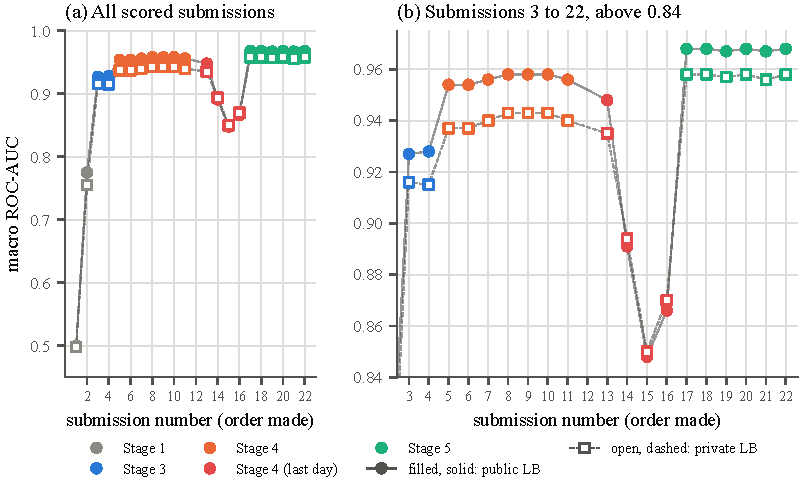
\includegraphics[width=\textwidth]{fig_leaderboard.pdf}
\caption[Leaderboard scores of all submissions]{Every submission made from the team's account, in order, with its public (filled) and private (open) score; stages as in Figure~\ref{fig:stages}, and submission 12 returned no score}
\label{fig:leaderboard}
\end{figure}

Several submissions of the last day scored lower than the picks. For these we relaxed our adoption rule and fitted separate blend weights for each finding on the 58 gold studies, which raised the gold score of the blend from 0.939 to 0.954. That gain was measured on the same 58 studies the weights were fitted to, so it was in-sample and meant little. For the same submissions we also fine-tuned the CoAtNet model for two epochs on Kaggle's GPUs (gold-58 0.924 against 0.923 before). To make room for more models, the blends also ran closer to the time limit. The results ranged from 0.948 down to 0.848 on the public leaderboard. For one of them the cause is known. It reached its internal deadline of 8.3 hours, and every study it had not reached received a constant default value. For the others the hidden-test logs are not visible to participants, so the cause could not be confirmed. None of these submissions was selected.

The team's final private score was \textbf{0.943}, from the better of the two picks, final-max v2, which contains R6; the fastMRI-free pick scored 0.940. This placed the team 490th of 6,299 teams on the private leaderboard, which earned a bronze medal; Kaggle's certificate is reproduced in Appendix~\ref{app:certificate}. The winning private score was 0.960. Our picks lost 0.015 between the public and the private leaderboard, against 0.010--0.011 for our own Stage~3 model and the later box-pooling model. The extra loss is consistent with, but does not prove, overfitting of the public blends to the public leaderboard.

% ----------------------------------------------------------------------
\subsection{Stage 5: Post-competition diagnosis and the improved model}
\label{sec:impl-post}

After the competition closed, the top teams published their methods and some of their code and labels. This made it possible to test, with controlled experiments, why our own model had stopped at 0.916 private.

\subsubsection{What the top solutions had in common} We read twelve published solutions. Their main points of agreement were: (1) labels made by LLM agents that look at the images as well as the report scored 0.93--0.95 against gold-58, far above our 0.890; (2) cropping and pooling each finding inside an anatomical region of interest added a further gain; (3) large ensembles added little; and (4) a single well-built model reached 0.954--0.958 on the private leaderboard. The first- and seventh-placed teams published their image-read labels \cite{tascj_agentlabels,songqizhou_llmlabels}, and the first-placed team also published its complete training code \cite{tascj_boxpool,tascj_roidetector,tascj_sideclassifier}.

\subsubsection{Measuring our labels} Figure~\ref{fig:labels}(a) compares our labels with the two image-read sets on the same 4,349 studies. Our report labels call MCL injury in 14.7\% of the studies against 2--3\% for the image readers, lateral OA in 23.5\% against 5--8\%, PF OA in 44.6\% against 19--22\%, and effusion in 59.4\% against 31--34\%. Reports mention small effusions and mild degenerative changes that an image reader working to a threshold would call negative. Against gold-58 the seventh-place labels scored 0.953 and the first-place labels 0.943; the latter were partly fitted to gold, so their score is in-sample (Figure~\ref{fig:labels}b). The two image-read sets disagree with each other on 1--10\% of the studies per finding, most often on synovitis (9.7\%), medial OA (8.9\%) and the medial meniscus (8.7\%).

\subsubsection{The label-swap experiment} To measure the effect of labels alone, we retrained our exact Stage~3 recipe (same fold, same seed, same code) and changed only the label file. Figure~\ref{fig:labelswap}(a) shows the result on gold-58. With our report labels the model scored 0.891; with the first-place labels 0.912 ($+0.021$, CI $[+0.004, +0.039]$); with the seventh-place labels 0.927 ($+0.036$, CI $[+0.018, +0.055]$); and with the mean of the two image-read sets 0.928. Synovitis alone rose from 0.689 to 0.857 with the seventh-place labels. Both gains were confirmed on our fold~0, where each model was scored against the image-read label set it had not been trained on: $+0.029$ and $+0.026$ over the model trained on our labels. This answers the question left open in Stage~2. Once the encoder was fine-tuned, the labels limited our model more than its design did.

\begin{figure}[htbp]
\centering\setstretch{1}
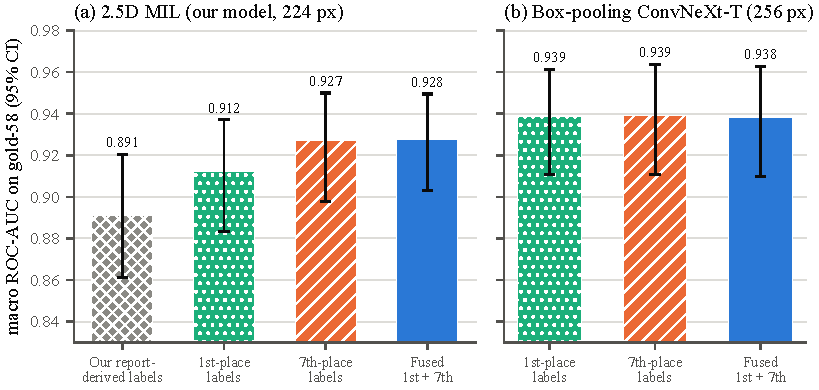
\includegraphics[width=\textwidth]{fig_label_swap.pdf}
\caption[Label-swap experiment on gold-58]{Label-swap experiment on gold-58 (95\% bootstrap CI): (a) our 2.5D model retrained with only the label file changed; (b) the box-pooling model trained with the same three image-read label choices}
\label{fig:labelswap}
\end{figure}

We also re-scored all the Stage~3 ablations against the image-read labels. The seed-to-seed spread on our fold~0 was about 0.007, and the higher resolution, six series, twelve epochs and the transformer head were all inside it. EfficientNetV2-S ($-0.018$) and mean pooling ($-0.013$) were worse by more than that spread. Under the image-read labels the higher-resolution version of our model (320-pixel crop, 0.365~mm per pixel) gained only $+0.003$ $[+0.001, +0.006]$ on our fold~0 and nothing on gold-58 (0.927 against 0.927), at 1.7 times the training time, so resolution was not pursued. An idea of our own, centring the predicted scores within each scanner group, lowered the score on our fold~0 from 0.926 to 0.917 and was dropped.

\subsubsection{Adopting the box-pooling architecture} With the image-read labels our model reached 0.927 on gold-58, roughly where the first-placed team's write-up places its own model before region-of-interest pooling, cropping and the auxiliary heads. Rebuilding those parts ourselves would have taken longer than the time available before the project presentation. We therefore adopted their published architecture (Section~\ref{sec:design-bp}) as the base and focused our own work on the labels, the training plan, the inference pipeline and the evaluation.

\subsubsection{Training on Kaggle} We wrote a builder that generates a training notebook from the published script with switches for the label file, fold, seed and time budget. It also saves validation predictions for every series and adds an inference-only switch for attention sharpening, described below. The runs used the free two-T4 quota of a team member's Kaggle account. Each run trained for eight epochs on about 19,200 series (2,400 updates per epoch) and took 5.4--6.1 hours of training, plus validation. The data loader waited only 1\% of the time while reading directly from Kaggle's network storage, so no image cache was needed. Six runs were made (Table~\ref{tab:bpruns}), all on the five-fold split of the published code. A0 and A1 differ only in the label set, A2 uses the fused labels of Equation~\eqref{eq:fused}, and C1--C3 repeat A2 on folds 1--3, so that the six models together cover different training subsets. Validation on gold-58 was recorded every epoch (Figure~\ref{fig:curves}b), but the last epoch was always used; gold was never used to choose an epoch.

\begin{table}[htbp]
\centering\footnotesize\setstretch{1}
\caption[Box-pooling training runs]{Box-pooling training runs (8 epochs each, Kaggle 2 $\times$ T4); gold-58 at the last epoch}
\label{tab:bpruns}
\begin{tabular}{C{1.1cm}L{4.4cm}C{1.1cm}C{2.0cm}C{2.4cm}}
\toprule
Run & Training labels & Fold & Gold-58 AUC & Training time (h) \\
\midrule
A0 & first-place image-read labels & 0 & 0.9388 & 5.5 \\
A1 & seventh-place image-read labels & 0 & 0.9389 & 5.7 \\
A2 & fused (mean of both) & 0 & 0.9383 & 5.4 \\
C1 & fused & 1 & 0.9369 & 5.7 \\
C2 & fused & 2 & 0.9433 & 6.1 \\
C3 & fused & 3 & 0.9397 & 5.6 \\
\midrule
\multicolumn{3}{l}{Mean of the six models} & 0.9409 & -- \\
\bottomrule
\end{tabular}
\end{table}

\subsubsection{Our inference pipeline} The published inference notebooks depended on TensorRT engines and a compiled reader tied to the authors' own weights, so we wrote our own inference script that runs the three published modules unchanged: side classifier, detector (with mirrored test-time averaging) and box-pooling classifiers. A series that cannot be read is skipped and reported, never filled with zeros. A series without detector boxes receives the median box of its plane, and a batch that fails, for example from running out of memory on a very long series, is repeated one series at a time. Locally it ran the three public test studies in 25~s, and on 16 gold studies its predictions matched the published notebook's own predictions for the same weights with a correlation of 0.996. Before any GPU time was spent, the notebook was rehearsed in a free CPU session on Kaggle with every multi-series batch forced to fail once; all 15 series were recovered by the one-at-a-time path and the run completed in 202~s.

\subsubsection{Results} The A0 versus A1 comparison was a tie: 0.9388 against 0.9389 on gold-58, and on the published fold~0 each model won by about 0.003 when scored against its own label source (Figure~\ref{fig:labelswap}b). The stronger architecture was much less sensitive to the label set than our own model had been, where the same swap had made a difference of 0.015. The fused labels gave a model between the two single-source models on every reference. Late submissions, which Kaggle scores on the private leaderboard but does not rank, gave the results in Table~\ref{tab:late}. Model A0, the published recipe trained unchanged on one fold, scored 0.955 private, which reproduces the 0.954 published for it and shows that our inference pipeline is sound. Training the same pipeline on the fused labels gave 0.958, a difference of the size that the leaderboard's own noise could produce. Every model or average of models trained on image-read labels scored 0.955--0.958 private, against 0.943 for our best submission during the competition and 0.960 for the winning team.

\begin{table}[htbp]
\centering\footnotesize\setstretch{1}
\caption[Late submissions of the box-pooling models]{Late submissions of the box-pooling models (scored after the competition, not ranked)}
\label{tab:late}
\begin{tabular}{L{6.3cm}C{2.0cm}C{2.0cm}L{2.6cm}}
\toprule
Models & Private & Public & Account \\
\midrule
A0 (first-place labels) & 0.955 & 0.963 & team member$^{*}$ \\
A1 (seventh-place labels) & 0.957 & 0.967 & team member$^{*}$ \\
A0 + A1 & 0.958 & 0.967 & team member$^{*}$ \\
A2 (fused labels) & 0.958 & 0.968 & both \\
A2 + C1 & 0.958 & 0.968 & team \\
A0 + A1 + A2 & 0.958 & 0.968 & team \\
A0 + A1 + A2 + C1 & 0.958 & 0.968 & team \\
A1 with attention sharpening $s=2$ & 0.956 & 0.967 & team \\
A1 with per-finding sharpening & 0.957 & 0.967 & team \\
\bottomrule
\multicolumn{4}{l}{\scriptsize $^{*}$ scores from the project's decision log; all other rows read from the Kaggle submission history.}
\end{tabular}
\end{table}

Before the last two folds were trained, we fixed in writing that the equal-weight mean of all six models would be reported as the final ensemble. This was done because picking the best of many variants by its leaderboard score would itself be a form of selection on the test set. The notebook for this six-model ensemble, built automatically when the last two runs finished, stopped with an error on Kaggle and was not scored at the time of writing. On gold-58 the six-model mean scores 0.941 $[0.912, 0.965]$, which we report as a description only. Figure~\ref{fig:gold} shows that it gains most on synovitis (0.877 against 0.680 for our Stage~3 model), effusion, ACL and the menisci, while our Stage~3 model remains better on lateral OA and bone contusion.

\subsubsection{Ideas that were tested and rejected} Four further ideas were examined on the published fold~0 before any leaderboard submission. Three were tested against a rule fixed in advance and one was only considered.
\begin{itemize}[leftmargin=1.4em]
\item \emph{Adding our own study-level model to the ensemble.} Trained with the published fold~0 held out, our model scored 0.957 alone against 0.968--0.971 for the box-pooling models, and adding it at one third weight changed the score by $-0.0012$ $[-0.0023, -0.0000]$. It was not added.
\item \emph{Attention sharpening.} Multiplying the in-box attention score $a$ of Equation~\eqref{eq:boxweight} by a factor $s$ at inference makes the pooling more ($s>1$) or less ($s<1$) focused. Two other teams had reported a gain from this in their own models. Figure~\ref{fig:sharpen} shows that the trained models already sit at their optimum: $s=1.25$ gained at most $+0.0007$, while $s=3$ lost 0.004--0.006. Focal findings such as medial OA and fractures gained slightly from sharpening, while diffuse findings, above all synovitis, lost. Two sharpened versions sent to the leaderboard as a check scored 0.956 and 0.957 private, against 0.957 for the unchanged model, so sharpening was not adopted.
\item \emph{Weighting series types.} Instead of the plain mean over a study's series, we fitted one weight per finding and series type (plane and fat suppression) with five-fold cross-fitting. The best setting gained $+0.0004$ to $+0.0007$, ten times smaller than the seed spread; with weaker regularisation the weights spread by a factor of 50 and the score fell. Fixed alternatives such as the maximum over series were worse, and the plain mean was kept.
\item \emph{Test-time flipping of the classifier.} Not tried for this model, because left knees are already mirrored before classification, and a related test in Stage~4 had lowered the score of a public model by 0.007.
\end{itemize}

\begin{figure}[htbp]
\centering\setstretch{1}
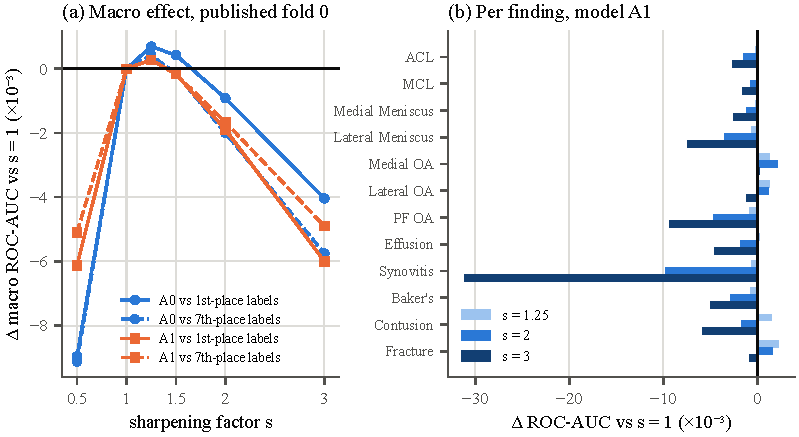
\includegraphics[width=\textwidth]{fig_sharpen.pdf}
\caption[Attention sharpening at inference]{Attention sharpening at inference on the 870 studies of the published fold 0: (a) change in macro AUC for models A0 and A1 scored against both image-read label sets; (b) change per finding for model A1 against the first-place labels}
\label{fig:sharpen}
\end{figure}

% ----------------------------------------------------------------------
\subsection{Stage 6: The local workstation}
\label{sec:impl-demo}

The last part of the project made the final models usable outside Kaggle. The workstation follows the design of Section~\ref{sec:design-demo}. A user drops a DICOM folder, a set of files or a zip archive onto the page. The browser packs the files and sends them to the local server, which parses the headers, groups the series, skips localisers and series with fewer than six slices, reads the fat-suppression setting from the header (it agreed with the dataset's own labels on 99\% of 600 training series) and places every slice in patient coordinates for the three-dimensional view. Inference then runs the side classifier, the detector and all six classifiers one series at a time and streams every intermediate result to the page as it is computed. Figure~\ref{fig:ws-overview} shows the screen after a run on one of the three public example test studies. The detector's box for the medial meniscus and the cells with positive evidence are drawn on the sagittal, coronal and axial views.

\begin{figure}[htbp]
\centering\setstretch{1}
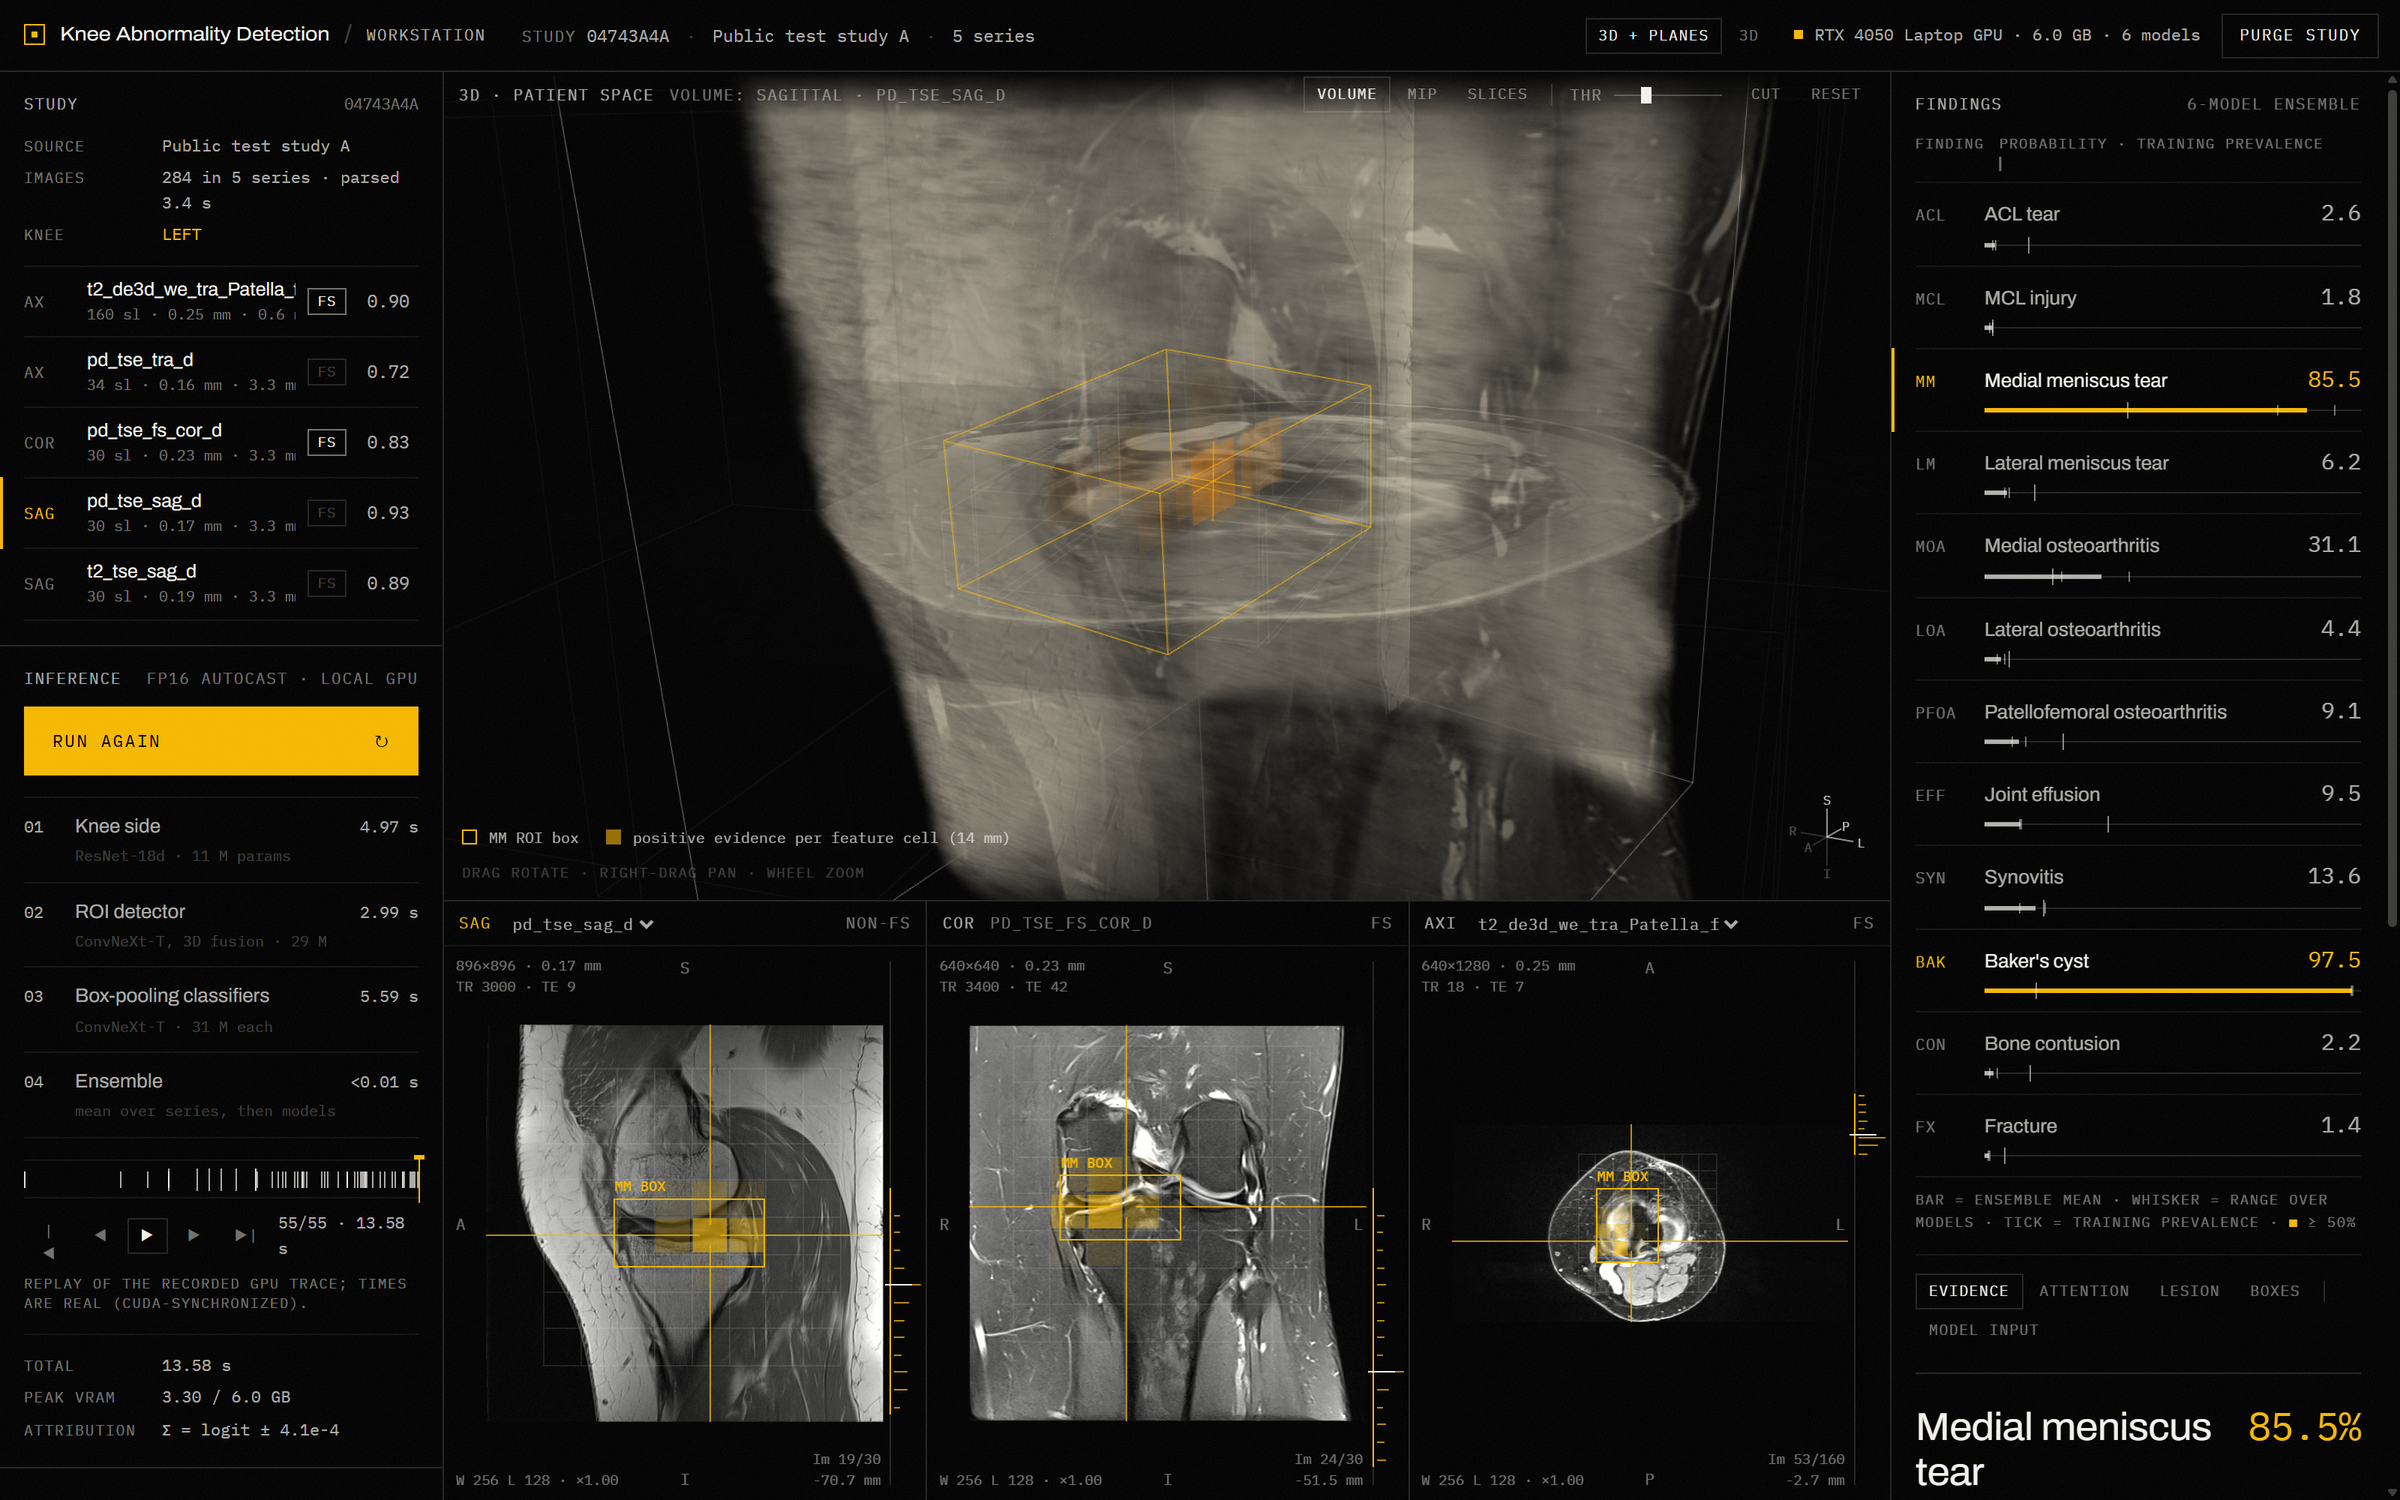
\includegraphics[width=\textwidth]{ws_overview.png}
\caption[The local workstation after inference]{The local workstation after inference on a public example study: series list and GPU trace on the left, the three-dimensional view and the three plane views with the medial meniscus box and evidence cells in the centre, the twelve findings with ensemble mean and model range on the right}
\label{fig:ws-overview}
\end{figure}

For each finding the page shows the ensemble probability, the spread across the six models, and the training prevalence for reference. Selecting a finding opens its detail panel (Figure~\ref{fig:ws-detail}b): the probability from each model, the probability from each series, and the slices that contributed most to the score. Four overlays can be laid over the images: the detector's box, the pooling weights, the evidence of Equation~\eqref{eq:attribution} averaged over the six models, and the output of the lesion head, which was trained to mark lesion cells but does not feed the probability, so it gives an independent second localisation. The panel states plainly that the evidence map shows what drove the score, which need not be the most visible lesion.

\begin{figure}[htbp]
\centering\setstretch{1}
\begin{minipage}[b]{0.40\textwidth}\centering
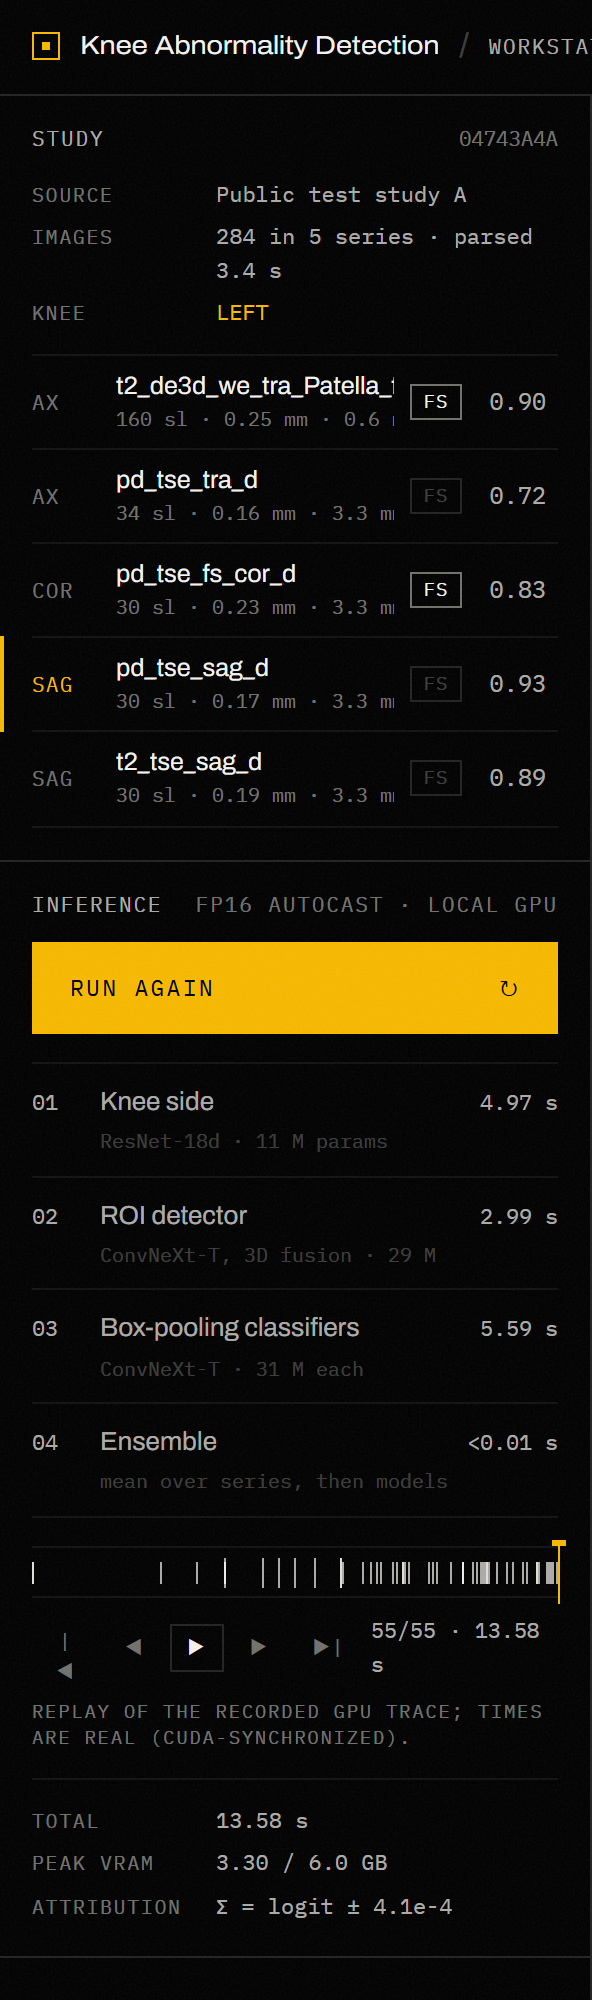
\includegraphics[height=16.5cm]{ws_left_panel.png}\\[2pt]
{\footnotesize\itshape (a) study, series and inference trace}
\end{minipage}\hfill
\begin{minipage}[b]{0.55\textwidth}\centering
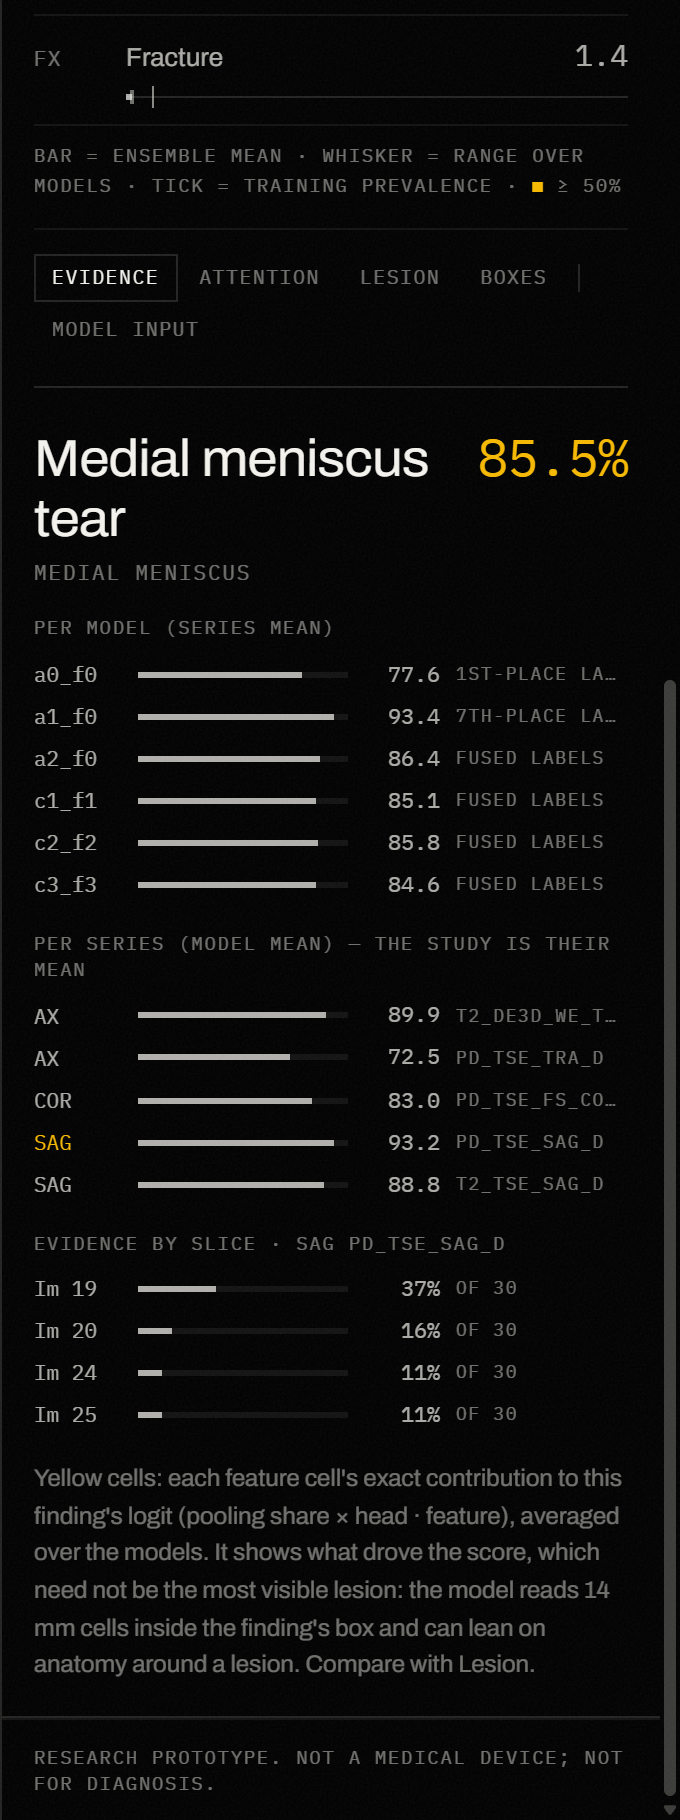
\includegraphics[height=16.5cm]{ws_findings_detail.png}\\[2pt]
{\footnotesize\itshape (b) detail of one finding}
\end{minipage}
\caption[Workstation panels]{Workstation panels: (a) the loaded series with the timed inference steps, peak GPU memory and the attribution check; (b) the per-model and per-series probabilities and the slices that contributed most to the medial meniscus score}
\label{fig:ws-detail}
\end{figure}

The workstation fits on the 6~GB laptop GPU. The weights of all eight networks take 863~MB and load in about 10~s. A typical study uses 1.2~GB of GPU memory at peak, and the largest series we tried, 160 slices of 640 $\times$ 1280 pixels, used 3.1~GB. A typical study takes 4--11~s once the GPU is warm. The study in Figure~\ref{fig:ws-detail} is a heavier case with a 160-slice three-dimensional series: the side classifier took 5.0~s, the detector 3.0~s and the six classifiers 5.6~s, 13.6~s in all, with a peak of 3.3~GB. No quantisation was needed, so the predictions are those of the Kaggle pipeline (Section~\ref{sec:testing}).

During testing, one team member noticed that the evidence for patellofemoral OA peaked on a different slice from the most visible dark lesion. We checked the slice mapping and found it correct, since the model's evidence for that finding really did peak on the patella. This was the reason the lesion overlay and the per-slice breakdown were added, so that a user can compare the two localisations directly.

% ----------------------------------------------------------------------
\section{Testing and Verification}
\label{sec:testing}

Testing in this project covered both the software and the reported results. Table~\ref{tab:tests} lists the main tests and their outcomes.

\begin{table}[htbp]
\centering\footnotesize\setstretch{1}
\caption{Tests and verification checks with their outcomes}
\label{tab:tests}
\begin{tabularx}{\textwidth}{C{0.8cm} L{3.6cm} Y L{2.5cm}}
\toprule
No. & Check & Method & Result \\
\midrule
T1 & Compressed DICOM decoding & training slices converted to JPEG-Lossless and JPEG~2000, decoded and compared & bit-identical \\
T2 & Inference failure handling & six local cases: normal run; damaged fluid-sensitive series; missing plane; missing decoders; mixed ensemble; damaged end and middle slices & fallback, mask, abort, mean, drop and reject as designed \\
T3 & Notebook end to end & each generated notebook run in a fresh interpreter, including the exact upload folder & valid submission files \\
T4 & Float16 on T4 & predictions compared with float32 & max $|\Delta p| = 0.0014$, Spearman $\geq 0.9998$ \\
T5 & Train/test preprocessing parity & same series through both code paths & bit-identical on 51 series \\
T6 & Slice ordering & monotonic positions in a 2,000-series sample & no violations \\
T7 & Single-pass rewrite (Stage 4) & rewritten stage against the separate stage on gold-58 & equal on 57 of 58 studies \\
T8 & Box-pooling inference script & our pipeline against the published notebook, 16 gold studies & correlation 0.996 \\
T9 & Kaggle rehearsal & CPU session, every batch forced to fail once & 15/15 series recovered, 202~s \\
T10 & Reproduction of a published result & model A0 late-submitted & 0.955 private vs 0.954 published \\
T11 & Sharpening switch & $s=1$ against the unmodified model & max difference 0.0 \\
T12 & Workstation fidelity & engine against the Kaggle inference script run locally with the same weights, 3 studies, 90 series--model pairs & max $|\Delta p| = 1.6\times10^{-4}$ \\
T13 & Attribution exactness & sum of cell contributions plus bias against the logit & $5\times10^{-7}$ (fp32), $\leq 0.05$ (fp16) \\
T14 & Sealed gold evaluation & scoring script writes a lock file first and refuses a second run & enforced \\
\bottomrule
\end{tabularx}
\end{table}

\paragraph{Software tests.} Tests T1--T6 were run before the Stage~3 submission. The decoder test (T1) matters because the hidden test set could not be inspected and its run log is not shown to participants, so a silent decoding failure would have been invisible. T4 shows that running in float16 on Kaggle's T4 GPUs changes the probabilities by at most 0.0014 and leaves their order practically unchanged, which is what the AUC depends on. T8--T10 together show that the post-competition inference pipeline reproduces the published model, first on the predictions of the published notebook and then on the private leaderboard. T12 was re-run after every change to the workstation engine; the remaining difference of $1.6\times10^{-4}$ comes from float16 rounding.

\paragraph{Verification of results.} Our own Stage~3 model was never selected on gold-58, and its gold predictions were sealed until the choice was fixed (T14). In Stage~5 no epoch or model was chosen on gold-58. The exceptions were in Stage~4, where public models and blends were compared on gold-58 and the last-day blends were fitted to it. Comparisons between our own models on the same studies are paired and carry bootstrap intervals; leaderboard scores and the single scores of public models do not. Every leaderboard score in Figure~\ref{fig:leaderboard} and Tables~\ref{tab:endgame} and \ref{tab:late} was read from the Kaggle submission history, apart from the three late-submission rows marked as coming from the project log. The figures in this report were drawn by scripts in the report folder from aggregate tables that those scripts compute from the project's run outputs.

\paragraph{Problems found by testing and operation.} Not every problem was caught by a test before it happened. Once, the scripts that polled Kaggle froze for about three hours while the laptop slept, and once two copies of a hand-over script ran at the same time for five hours because stopping the parent process did not stop its child shells; they submitted the same notebook twice. The scripts were rewritten as single processes with a state file and a request to Windows to stay awake. On the last day of the competition, as described in Section~\ref{sec:impl-endgame}, submissions that ran close to the nine-hour limit produced low scores. Both lessons fed into the post-competition work, where run time was budgeted with a margin and every automatic step was made safe to repeat.

\paragraph{Summary of results.} Table~\ref{tab:summary} brings together the main measured results of the project.

\begin{table}[htbp]
\centering\footnotesize\setstretch{1}
\caption{Summary of the main results (macro AUC)}
\label{tab:summary}
\begin{tabular}{L{6.6cm}C{1.9cm}C{1.9cm}C{1.9cm}}
\toprule
System & Gold-58 & Public LB & Private LB \\
\midrule
Frozen EfficientNet-B0, own DICOM pipeline (Stage 1) & 0.753$^{\dagger}$ & 0.775 & 0.755 \\
Fine-tuned 2.5D MIL ensemble F1--F3, report labels (Stage 3) & 0.906 & 0.927 & 0.916 \\
Final competition picks, public models (Stage 4) & -- & 0.958 & 0.943 \\
2.5D MIL, fused image-read labels, one fold (Stage 5) & 0.928 & -- & -- \\
Box-pooling, fused labels, one model A2 (Stage 5) & 0.938 & 0.968 & 0.958 \\
Box-pooling, mean of A0, A1, A2 and C1 (Stage 5) & -- & 0.968 & 0.958 \\
Box-pooling, mean of six models (Stage 5) & 0.941 & not scored & not scored \\
Winning team of the competition & -- & -- & 0.960 \\
\bottomrule
\multicolumn{4}{l}{\scriptsize $^{\dagger}$ the frozen-feature design re-run under the Stage 3 protocol (E0).}
\end{tabular}
\end{table}
